\documentclass[tikz,border=1.5pt]{standalone}
\newif\ifko \kofalse

% style.tex — 구성도 공용 (standalone, xelatex). \kotrue / \kofalse 를 먼저 정함.
\usepackage{mathptmx}
\usepackage[no-math]{fontspec}
\setmainfont{TeX Gyre Heros}
\ifko
  \newfontfamily\krfont{Noto Sans CJK KR}[Scale=0.9]
  \usepackage[Latin,Korean]{ucharclasses}
  \setTransitionsForKorean{\begingroup\krfont}{\endgroup}
\fi
\usepackage{xcolor}
\definecolor{cFRiii}{HTML}{0072B2}
\definecolor{cFRv}{HTML}{D55E00}
\definecolor{cEmph}{HTML}{009E73}
\usepackage{tikz}
\usetikzlibrary{positioning,fit,backgrounds,arrows.meta,calc,shapes.geometric,shapes.misc,decorations.pathreplacing}
\newcommand{\T}[2]{\ifko #1\else #2\fi}
\tikzset{
  >={Stealth[length=2.2mm,width=1.6mm]},
  every node/.style={font=\fontsize{7.2}{8.6}\selectfont},
  box/.style={draw=black, line width=0.5pt, rounded corners=1.2pt, fill=white, align=center, inner sep=2.6pt, minimum height=8.5mm, text width=#1},
  box/.default=24mm,
  gbox/.style={box=#1, fill=black!6},
  gbox/.default=24mm,
  ebox/.style={box=#1, draw=cEmph, line width=1.0pt, fill=cEmph!7},
  ebox/.default=24mm,
  grp/.style={draw=black!55, dashed, line width=0.45pt, rounded corners=2pt, inner sep=3.2mm},
  grplabel/.style={anchor=north west, font=\fontsize{7.6}{9}\selectfont\bfseries, inner sep=1.2pt, fill=white},
  ar/.style={->, line width=0.6pt},
  ear/.style={->, line width=1.1pt, draw=cEmph},
  dar/.style={->, line width=0.55pt, dashed},
  small/.style={font=\fontsize{6.3}{7.4}\selectfont},
  lab/.style={font=\fontsize{6.3}{7.4}\selectfont, fill=white, inner sep=1pt},
}
\newcommand{\D}{\fontsize{6.3}{7.5}\selectfont\color{black!78}}
\newcommand{\code}[1]{\texttt{#1}}

\begin{document}
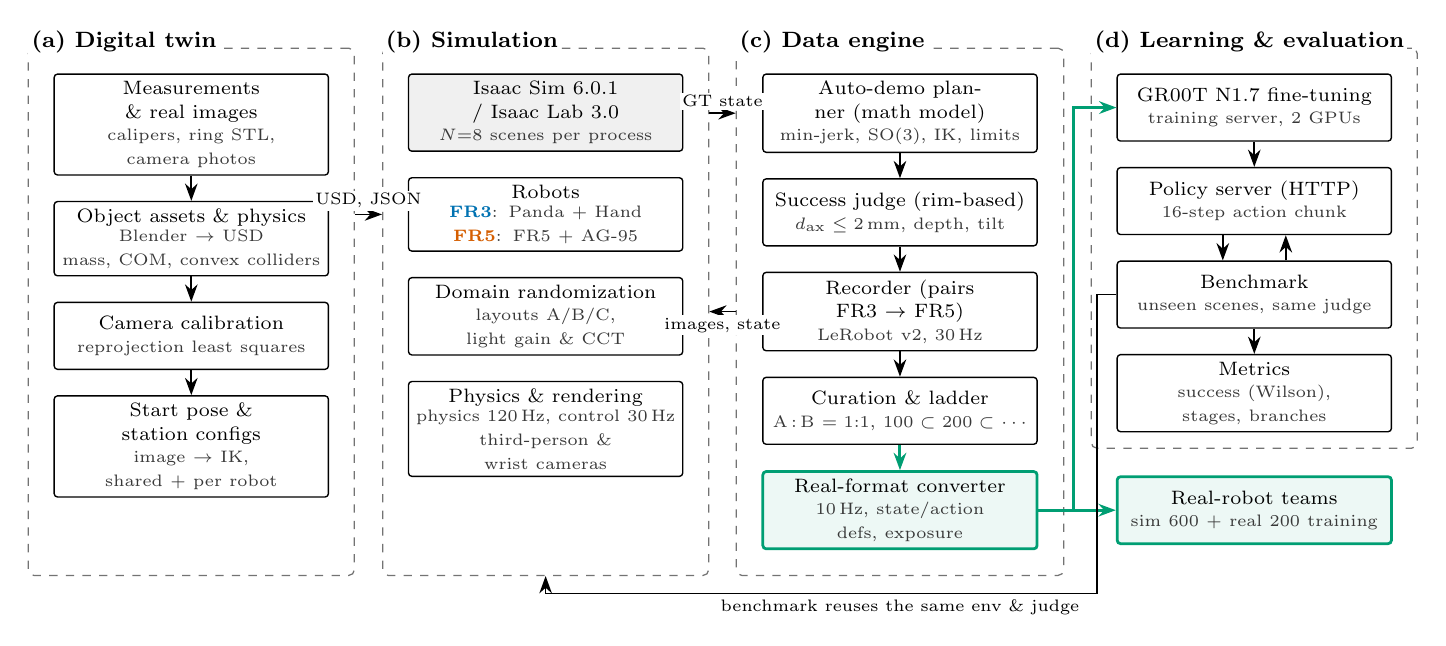
\begin{tikzpicture}[node distance=3.2mm]
\def\W{33mm}
% ---------------- 1 디지털 트윈
\node[box=\W, anchor=north] (m1) at (0,0) {\T{실측 · 실물 화면}{Measurements \& real images}\\[-0.5pt]{\D\T{캘리퍼 치수, 링 STL, 카메라 사진}{calipers, ring STL, camera photos}}};
\node[box=\W, below=of m1] (m2) {\T{물체 모양 · 물리}{Object assets \& physics}\\[-0.5pt]{\D Blender $\rightarrow$ USD\\\T{질량 $\cdot$ 무게중심 $\cdot$ 볼록 충돌체}{mass, COM, convex colliders}}};
\node[box=\W, below=of m2] (m3) {\T{카메라 맞추기}{Camera calibration}\\[-0.5pt]{\D\T{재투영 최소제곱}{reprojection least squares}}};
\node[box=\W, below=of m3] (m4) {\T{시작 자세 · 실험대 설정}{Start pose \& station configs}\\[-0.5pt]{\D\T{화면 $\rightarrow$ 역기구학, 공용 + 로봇별}{image $\rightarrow$ IK, shared + per robot}}};
% ---------------- 2 Isaac Sim / Lab
\node[gbox=\W, anchor=north] (e1) at ($(m1.north)+(45mm,0)$) {Isaac Sim 6.0.1 / Isaac Lab 3.0\\[-0.5pt]{\D\T{한 프로세스에 장면 $N{=}8$}{$N{=}8$ scenes per process}}};
\node[box=\W, below=of e1] (e2) {\T{로봇}{Robots}\\[-0.5pt]{\D\textcolor{cFRiii}{\textbf{FR3}}: Panda + Hand\\\textcolor{cFRv}{\textbf{FR5}}: FR5 + AG-95}};
\node[box=\W, below=of e2] (e3) {\T{도메인 랜덤화}{Domain randomization}\\[-0.5pt]{\D\T{배치 A $\cdot$ B $\cdot$ C, 조명 밝기 $\cdot$ 색온도}{layouts A/B/C, light gain \& CCT}}};
\node[box=\W, below=of e3] (e4) {\T{물리 $\cdot$ 렌더링}{Physics \& rendering}\\[-0.5pt]{\D\T{물리 120 Hz, 제어 30 Hz}{physics 120\,Hz, control 30\,Hz}\\\T{3인칭 $\cdot$ 손목 카메라}{third-person \& wrist cameras}}};
% ---------------- 3 데이터 엔진
\node[box=\W, anchor=north] (d1) at ($(m1.north)+(90mm,0)$) {\T{자동 시연기 (수학 모델)}{Auto-demo planner (math model)}\\[-0.5pt]{\D\T{최소 저크, SO(3), 역기구학}{min-jerk, SO(3), IK, limits}}};
\node[box=\W, below=of d1] (d2) {\T{성공 판정 (턱 기준)}{Success judge (rim-based)}\\[-0.5pt]{\D $d_{\mathrm{ax}}\!\le\!2$\,mm, \T{깊이, 기울기}{depth, tilt}}};
\node[box=\W, below=of d2] (d3) {\T{기록 (짝: FR3 $\rightarrow$ FR5)}{Recorder (pairs FR3 $\rightarrow$ FR5)}\\[-0.5pt]{\D LeRobot v2, 30\,Hz}};
\node[box=\W, below=of d3] (d4) {\T{선별 $\cdot$ 사다리}{Curation \& ladder}\\[-0.5pt]{\D A\,:\,B $=1{:}1$, $100 \subset 200 \subset \cdots$}};
\node[ebox=\W, below=of d4] (d5) {\T{실물 형식 변환}{Real-format converter}\\[-0.5pt]{\D 10\,Hz, \T{상태 $\cdot$ 행동 정의, 노출}{state/action defs, exposure}}};
% ---------------- 4 학습 · 평가
\node[box=\W, anchor=north] (l1) at ($(m1.north)+(135mm,0)$) {\T{GR00T N1.7 미세조정}{GR00T N1.7 fine-tuning}\\[-0.5pt]{\D\T{학습 서버, GPU 2장}{training server, 2 GPUs}}};
\node[box=\W, below=of l1] (l2) {\T{정책 서버 (HTTP)}{Policy server (HTTP)}\\[-0.5pt]{\D\T{행동 묶음 16칸}{16-step action chunk}}};
\node[box=\W, below=of l2] (l3) {\T{벤치마크}{Benchmark}\\[-0.5pt]{\D\T{처음 보는 장면, 같은 판정}{unseen scenes, same judge}}};
\node[box=\W, below=of l3] (l4) {\T{지표}{Metrics}\\[-0.5pt]{\D\T{성공률 (Wilson), 단계, 갈래}{success (Wilson), stages, branches}}};
\node[ebox=\W, anchor=center] (l5) at (l1.center |- d5.center) {\T{실물 팀}{Real-robot teams}\\[-0.5pt]{\D\T{시뮬 600 + 실물 200 학습}{sim 600 + real 200 training}}};
% ---------------- 묶음
\begin{scope}[on background layer]
\coordinate (BOT) at ($(d5.south)+(0,0)$);
\node[grp, fit=(m1)(m4)(m1.north |- BOT)] (G1) {};
\node[grp, fit=(e1)(e4)(e1.north |- BOT)] (G2) {};
\node[grp, fit=(d1)(d5)] (G3) {};
\coordinate (L1T) at ($(l1.north)+(0,1.2mm)$);
\node[grp, inner ysep=2mm, fit=(l1)(l4)(L1T)] (G4) {};
\end{scope}
\node[grplabel] at ($(G1.north west)+(0,2.6mm)$) {(a) \T{디지털 트윈}{Digital twin}};
\node[grplabel] at ($(G2.north west)+(0,2.6mm)$) {(b) \T{시뮬 환경}{Simulation}};
\node[grplabel] at ($(G3.north west)+(0,2.6mm)$) {(c) \T{데이터 엔진}{Data engine}};
\node[grplabel] at ($(G4.north west)+(0,2.6mm)$) {(d) \T{학습 $\cdot$ 평가}{Learning \& evaluation}};
% ---------------- 화살표
\foreach \a/\b in {m1/m2,m2/m3,m3/m4,d1/d2,d2/d3,d3/d4,l1/l2,l3/l4} \draw[ar] (\a) -- (\b);
\draw[ear] (d4) -- (d5);
\draw[ar] (G1.east |- e2) -- node[lab, above, yshift=1pt]{USD, JSON} (G2.west |- e2);
\draw[ar] (G2.east |- d1) -- node[lab, above, yshift=1pt]{\T{정답 상태}{GT state}} (G3.west |- d1);
\draw[ar] (G3.west |- d3) -- node[lab, below, yshift=-1pt]{\T{화면 $\cdot$ 상태}{images, state}} (G2.east |- d3);
\draw[ear] (d5.east) -- ++(4.5mm,0) |- (l1.west);
\draw[ear] (d5.east) -- (l5.west);
\draw[ar] ([xshift=-4mm]l2.south) -- ([xshift=-4mm]l3.north); \draw[ar] ([xshift=4mm]l3.north) -- ([xshift=4mm]l2.south);
\draw[ar] (l3.west) -- ++(-2.5mm,0) |- ($(G3.south east)+(0,-2.2mm)$) -| (G2.south);
\node[lab, anchor=north] at ($(G3.south)+(0,-2.6mm)$) {\T{벤치는 같은 환경 $\cdot$ 판정을 씀}{benchmark reuses the same env \& judge}};
\end{tikzpicture}
\end{document}
